\documentclass[pdflatex,sn-mathphys-num]{sn-jnl}
\usepackage{graphicx,amsmath,amssymb,booktabs,tabularx,url,microtype,etoolbox}
\raggedbottom
\AtBeginDocument{\let\burl\url}
\makeatletter
% Keep the complete structured abstract together without changing type sizes.
\patchcmd{\@maketitle}{\vskip21pt}{\vskip0pt}{}{\errmessage{Title spacing patch failed}}
\patchcmd{\@maketitle}{\vskip24pt}{\vskip12pt}{}{\errmessage{Address spacing patch failed}}
\patchcmd{\@maketitle}{\vskip24pt}{\vskip12pt}{}{\errmessage{Email spacing patch failed}}
\def\ps@paper{\let\@oddhead\@empty\let\@evenhead\@empty
  \def\@oddfoot{\hfil\thepage\hfil}\let\@evenfoot\@oddfoot}
\let\ps@titlepage\ps@paper
\let\ps@headings\ps@paper
\makeatother
\pagestyle{paper}
% All numerical claims are expanded into generated fragments.

\begin{document}
\title[Crowd supervision and selective prediction]{Crowd Supervision and Vocabulary-Mismatched Selective Facial-Expression Prediction}
\author[1]{\fnm{Gunjan Kumar} \sur{Mishra}}\email{mgunjan67@gmail.com}
\author[2]{\fnm{Bijaya} \sur{Ghimire}}\email{vijay.gh74@gmail.com}
\author*[3]{\fnm{Badri Raj} \sur{Lamichhane}}\email{d6622300231@g.siit.tu.ac.th}
\author[4]{\fnm{Alan} \sur{Shah}}\email{shahalan0202@gmail.com}
\affil[1]{\orgname{WorldQuant University}, \orgaddress{\city{Washington, D.C.}, \country{United States}}}
\affil[2]{\orgdiv{Department of Electronics and Computer Engineering}, \orgname{Institute of Engineering, Paschimanchal Campus}, \orgaddress{\city{Pokhara}, \country{Nepal}}}
\affil*[3]{\orgdiv{School of Information, Computer and Communication Technology}, \orgname{Sirindhorn International Institute of Technology, Thammasat University}, \orgaddress{\city{Pathum Thani}, \country{Thailand}}}
\affil[4]{\orgname{Herald College Kathmandu}, \orgaddress{\city{Kathmandu}, \country{Nepal}}}
\abstract{\textbf{Purpose:} To test whether detailed crowd-vote distributions improve selective facial-expression prediction beyond simpler target softening, and diagnose reliability when prediction and annotation vocabularies differ. \textbf{Methods:} Twelve channel-gated Swin-T runs compare hard, tie-aware hard, dominant-confidence-preserving uniform-minority, and full soft targets across three matched seeds. Exact-pixel isolation separates training, checkpoint selection, calibration, and testing. Selected and fixed-epoch checkpoints are evaluated. Complete-vote disagreement is partitioned into unsupported mass, supported ambiguity, and excess error; calibration half-splits and a conservative fixed-grid comparator examine threshold transfer. \textbf{Results:} At 80\% coverage on 3,275 test images, mean disagreement is 26.30\% (hard), 25.82\% (tie-aware), 24.06\% (uniform-minority), and 23.68\% (soft). Soft minus uniform-minority is -0.38 percentage points (conditional 95\% pixel-cluster interval [-0.64, -0.07]). The test annotation floor exceeds calibration's by 2.97 percentage points, including 2.15 points of unsupported mass. \textbf{Conclusion:} Full soft targets yielded lower selective disagreement than the ambiguity-preserving uniform-minority control under this matched protocol. Confidence interpretation depends on the vote vocabulary and retained population. Findings concern one reused image source, not independent-domain reliability or communication benefit.
}
\keywords{facial-expression recognition, crowd annotations, selective prediction, label distributions, supported vote mass, confidence calibration}
\maketitle

\section{Introduction}
Crowd annotations make facial-expression recognition a distributional problem: people can assign different categories to the same image. A categorical reference conceals that disagreement, while a confidence-based selector can retain less ambiguous images without improving category choice. These issues become coupled when the predictor's output vocabulary omits categories included in the annotation panel. A low selected error against dominant labels need not imply low disagreement with the complete vote distribution.

Our sender-controlled expression-cue prototype motivates this measurement problem but is not its validation setting. Related applications include EmotionPush's text-based notifications \cite{wang2016emotionpush}, EmoChat's facial and textual signals \cite{chong2019emochat}, and expression-informed emoji selection \cite{liu2019selfawareness}. Before claiming any benefit during messaging, it is useful to establish what benchmark confidence and annotation agreement can support. Here we study that narrower reliability question.

A facial-expression category is not a direct observation of internal emotion, intention, or sincerity. Context, culture, individual differences, and deliberate expression constrain that inference \cite{barrett2019emotions}. Accordingly, the application suggests a fallible visual category, requires a per-message choice, and does not infer what the text means. The benchmark analysis concerns consistency with image annotations, not correctness about a person's feelings.

We ask three questions. RQ1: does the detailed allocation of minority votes add selective-prediction value beyond image-specific target softening, and does arbitrary tie resolution explain the hard/soft contrast? RQ2: how much selected disagreement comes from unsupported votes, supported-category ambiguity, and excess category-choice error? RQ3: what do calibration/test distribution diagnostics, calibration half-splits, and a conservative threshold comparator reveal about empirical target overshoot?

The contribution is a bounded empirical investigation of these alternative explanations, not a new architecture, loss principle, or decomposition theorem. Twelve matched training runs, selected versus fixed-epoch evaluation, and sample-level reliability diagnostics connect supervision choices to the meaning of the selected risk. The local messaging prototype supplies motivation and an implementation artifact, not application evidence. The initial six hard/soft runs preceded the review; the six control runs and follow-up endpoints were specified after those results were known and before the controls were trained. All analyses reuse the same image source and are not independent confirmation.

\section{Related work}
FER2013 supplies seven expression categories for low-resolution face images \cite{goodfellow2013fer}. FER+ adds multiple annotations for the same images, including contempt, unknown, and not-a-face responses \cite{barsoum2016ferplus}. Barsoum et al. already compare hard-label and distribution-based training methods. We build on that established learning principle by evaluating selective vote disagreement under matched supervision and isolated operational roles. We retain seven model outputs for compatibility with the prototype while accounting for all ten annotation categories in evaluation; our scores are not a replication of the original eight-expression FER+ benchmark.

Uncertain annotations have motivated FER-specific methods such as Self-Cure Network, which uses weighting and relabeling \cite{wang2020scn}. Our comparison instead changes the target representation of the same supported votes. Swin Transformer supplies hierarchical shifted-window features \cite{liu2021swin}, and channel recalibration follows the established squeeze-and-excitation principle \cite{hu2018senet}. The architecture is held fixed so that supervision is the experimental variable.
Vats and Chadha have also described Swin with squeeze-and-excitation for FER (unpublished preprint, 2023, \url{https://arxiv.org/abs/2301.10906}).

More recent distribution-learning approaches exploit additional structure. Le et al. construct uncertainty-aware target distributions using neighbors in valence--arousal space \cite{le2023uncertainty}. MIDAS extends mixup to soft-labeled facial-expression videos \cite{kawamura2024midas}. Our study neither implements those mechanisms nor compares against their reported benchmark scores. It uses observed static-image votes directly to examine a matched supervision contrast and its selective outcomes.

Selective classification examines the trade-off between rejection and error \cite{geifman2017selective}; SelectiveNet learns a rejector jointly with prediction \cite{geifman2019selectivenet}. We use the simpler maximum-probability score to isolate the supervision comparison. This does not establish superiority over learned selectors. Softmax scores need not be calibrated probabilities \cite{guo2017calibration}; an empirically fitted error target is not a guaranteed risk bound. Our reporting separates same-coverage ranking comparisons, calibration-fitted operating points, and disagreement inherent in the finite crowd annotations.

A closely related unpublished preprint by Wang, Li, and Wang combines vote-count modeling, predicted disagreement, and rejection for dynamic expressions (2026, \url{https://arxiv.org/abs/2609.17130}). Our static-image study addresses simpler target-representation controls and vocabulary diagnostics; it does not benchmark or claim priority over that framework.

\section{Methods}
\subsection{Data provenance and isolated roles}
FER2013 contains 28,709 Training, 3,589 PublicTest, and 3,589 PrivateTest rows. The CSV was acquired on 20 September 2026 from Kaggle mirror \texttt{deadskull7/fer2013}, version 1, rather than an official maintainer distribution. FER+ annotations were obtained from the official repository and joined using original row identifiers and partition checks. Online Resource 1 records immutable sources, hashes, and row-level manifests. Images are not redistributed; a mirror's advertised license does not independently establish rights to its underlying photographs.

The join follows the official FER+ conversion script's row indexing, not its potentially blank or duplicated output filenames. A separate raw-source audit checks all 35,887 original emotion IDs, pixel byte hashes, and partition positions against the retained manifest. Named vote columns are reordered to the canonical model classes. These checks establish internal consistency with the acquired archive, not independent authenticity or correctness of every annotation.

Exact pixel hashes define the operational roles in Table~\ref{tab:roles} and Fig.~\ref{fig:design}. We keep the Training rows unchanged. After removing 280 PublicTest rows matching Training pixels, the remaining pixel clusters are assigned to checkpoint selection or calibration by a fixed hash rule, without consulting labels or outcomes. The primary test population removes 314 PrivateTest rows whose pixels occur in Training or any PublicTest row. No exact pixels are shared across the four roles. This is not verified person-disjoint or near-duplicate-disjoint evaluation. Full PrivateTest predictions are retained for audit; all main follow-up comparisons use the isolated primary population.
\begin{table}[t]
\caption{Operational roles after exact-pixel isolation. Counts are images, not people}\label{tab:roles}
\centering\begin{tabular}{lrl}\toprule
Source and role & Images & Use\\\midrule
Training & 28,709 & Optimization\\
PublicTest: selection & 1,667 & Checkpoint choice\\
PublicTest: calibration & 1,642 & Threshold choice\\
PrivateTest: primary & 3,275 & Main evaluation\\
PrivateTest: full & 3,589 & Prediction archive\\
\bottomrule\end{tabular}\end{table}

\begin{figure}[t]
\centering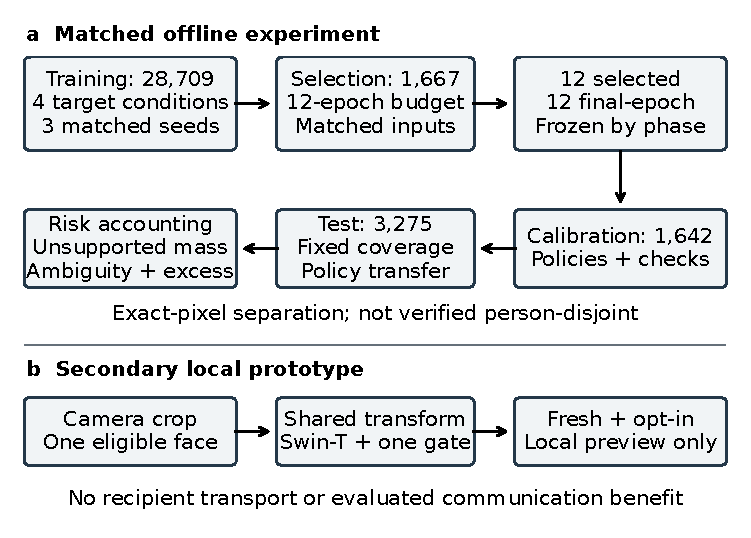
\includegraphics[width=\linewidth]{reviewer_followup/figures/Fig1.pdf}
\caption{Separate experimental and application flows. Checkpoint selection does not use the calibration subset; calibrated thresholds are evaluated offline and are not installed as a validated runtime guarantee. The application ends in a local preview, without recipient transport}\label{fig:design}
\end{figure}

\subsection{Matched hard and soft supervision}
Let $q_{ic}$ be the fraction of annotations for image $i$ assigned to category $c$, normalized over all ten categories. The first seven correspond to the supported expression outputs. Define supported mass $w_i=\sum_{c=1}^{7}q_{ic}$ and $r_{ic}=q_{ic}/w_i$ when $w_i>0$. For model probabilities $p_{ic}$, the two per-image objectives are
\begin{align}
\ell_i^{\mathrm{hard}}&=-w_i\log p_{i h_i},\quad h_i=\arg\max_{c\leq7}r_{ic},\\
\ell_i^{\mathrm{soft}}&=-w_i\sum_{c=1}^{7}r_{ic}\log p_{ic}
                     =-\sum_{c=1}^{7}q_{ic}\log p_{ic}.
\end{align}
All conditions use the same images and weights. The 152 Training rows with zero supported mass contribute zero supervised loss rather than an invented category. Among positive-mass rows, 1,360 have tied maximum votes; the original hard condition resolves ties by fixed class order. Losses are averaged over batch size, not divided by total supported mass.

Two controls address what the original contrast cannot isolate. The ambiguity-preserving uniform-minority condition (Uniform) retains $m_i=\max_c r_{ic}$ at the canonical dominant class $h_i$, but assigns $(1-m_i)/6$ to each other class. The tie-aware hard condition (Tie-hard) assigns $1/|T_i|$ to each member of $T_i=\{c:q_{ic}=\max_{k\leq7}q_{ik}\}$ and zero otherwise. Both minimize $-w_i\sum_c t_{ic}\log p_{ic}$. Uniform tests detailed minority allocation beyond image-dependent softening; it is not constant label smoothing and retains the canonical convention for tied maxima. Tie-hard is the expected loss under uniform random resolution among tied maxima, without additional random draws. It equals Hard on every unique-maximum image. These comparisons do not test discarding ambiguous images, manual relabeling, or training an expanded output vocabulary.

\subsection{Architecture, preprocessing, and optimization}
All conditions use torchvision Swin-T with ImageNet-1K V1 initialization \cite{liu2021swin,deng2009imagenet,paszke2019pytorch}. Its pooled feature $z\in\mathbb{R}^{768}$ is gated once, after the backbone:
\begin{equation}
\tilde z=z\odot\sigma\!\left(W_2\operatorname{ReLU}(W_1z)\right),
\quad W_1\in\mathbb{R}^{48\times768},\quad W_2\in\mathbb{R}^{768\times48}.
\end{equation}
The two gate layers omit biases; a biased linear layer produces seven logits. The gate adds 73,728 parameters. It is held fixed across the comparison, so the experiment cannot establish that gating is necessary or superior to another head.
A dimensioned head schematic and an illustrative composition interface are supplied in Online Resource 1.

Images are converted to grayscale, replicated across three channels, resized to $224\times224$ using bilinear interpolation, and normalized with mean and standard deviation 0.5. The canonical output order is angry, disgust, fear, happy, neutral, sad, and surprise. Horizontal flips are the only augmentation; they are keyed deterministically to seed, epoch, and original row. Seeds 17, 42, and 89 produce three matched groups of four conditions with identical within-seed initialization, sample order, augmentation, architecture, and budget. After model construction, the classifier is reset with Torch seed $1000+\mathrm{seed}$. Initial-state hashes and configuration comparisons verify the match between original and control runs.

All backbone and head parameters are optimized for 12 epochs with AdamW \cite{loshchilov2019adamw}, batch size 32, learning rate $10^{-4}$, weight decay $10^{-4}$, and a cosine scheduler with $T_{\max}=12$ and $\eta_{\min}=10^{-6}$, stepped after each epoch. AdamW uses $\beta_1=0.9$, $\beta_2=0.999$, and $\epsilon=10^{-8}$. Training uses BF16 autocast on an NVIDIA RTX 3070 Laptop GPU with 8 GB memory, PyTorch 2.8.0+cu128, and torchvision 0.23.0+cu128. Deterministic algorithms and seeded data loaders control this execution, not arbitrary cross-platform numerical behavior. The fixed budget is not a convergence or hyperparameter-optimality claim.

Checkpoint selection minimizes mean squared distance from the full ten-category vote distribution on the selection subset, with the seven predicted probabilities padded by three zeros. Earlier epochs win ties. This common criterion avoids selecting one condition by original-label F1. Each six-run phase is frozen before its calibration and test inference; original hard/soft results were known when the control protocol was written. Selected and fixed epoch-12 checkpoints are evaluated for all four conditions. The latter removes selection as a stopping decision but does not reconstruct selection by an alternative metric, because all historical intermediate weights were not retained. Both sets of weights, logs, and probabilities are released.
For fixed annotations, the squared distance differs from expected multiclass Brier loss against one annotation draw by $1-\lVert q_i\rVert_2^2$, a model-independent constant. Thus, it provides a common probability-sensitive selection objective rather than privileging either categorical reference.

Nevertheless, the constrained quadratic and training objectives have different ideal targets. For one image with $w>0$, weighted soft cross-entropy is minimized by $p_c=q_c/w$. Minimizing the ten-category squared distance under $\sum_{c\leq7}p_c=1$ instead gives $p_c=q_c+(1-w)/7$, by the quadratic's Lagrange multiplier. The solution is nonnegative and sums to one. These targets coincide at $w=1$, but generally differ otherwise. The score remains legitimate; the mismatch motivates the fixed-epoch and supported-mass diagnostics rather than an assertion of criterion neutrality.

\subsection{Disagreement, annotation floor, and classification metrics}
For predicted category $\hat c_i=\arg\max p_i$, expected disagreement with one draw from the empirical annotations is $d_i=1-q_{i\hat c_i}$. It is not a claim about emotional truth. The best available seven-category prediction has floor $b_i=1-\max_{c\leq7}q_{ic}$, giving
\begin{equation}
d_i=b_i+e_i,\qquad e_i=\max_{c\leq7}q_{ic}-q_{i\hat c_i}\geq0.
\label{eq:decomposition}
\end{equation}
The floor includes both disagreement among supported categories and votes outside the model's vocabulary. We report the mean floor and excess $e_i$ on the same accepted images as the total disagreement. They distinguish selecting less ambiguous images from choosing better categories, without treating the finite crowd distribution as a population oracle. Ten-category squared distribution distance additionally evaluates probability allocation, not just the winning category.

We further separate the floor using an accounting identity, not a new theorem:
\begin{equation}
d_i=\underbrace{1-w_i}_{\text{unsupported mass}}+
\underbrace{w_i-\max_{c\leq7}q_{ic}}_{\text{supported ambiguity}}+e_i.
\label{eq:threeparts}
\end{equation}
If an ideal model has $p_i=r_i$, its disagreement is $1-w_i\max_c p_{ic}$. Maximum softmax probability (MSP) alone omits $w_i$: an MSP of 0.9 implies disagreement 0.1 when $w_i=1$, but 0.55 when $w_i=0.5$. This is a hypothetical consequence of the definitions, not evidence that omitted mass alone caused the observed transfer failure. Annotation-derived $w_i$ is unavailable for a new runtime image and is never used as a deployable selector here.

We report $w=0$, $0<w<1$, and $w=1$ strata. Restricting each model's global 80\% accepted set differs from separately selecting 80\% within each stratum; both are labeled. For positive-mass images, $1-r_{i\hat c_i}$ is additionally reported as supported-only disagreement. This conditional endpoint changes the reference population of votes and is not a replacement for complete-vote risk or an expanded-vocabulary experiment.

Weighted and macro F1 against original FER2013 labels are secondary reference-specific diagnostics \cite{sokolova2009metrics}. Weighted F1 is $\sum_c n_c F1_c/N$; macro F1 averages the seven $F1_c$ values equally, assigning zero to undefined class scores. Crowd-majority weighted F1 uses only images with more than half of all votes assigned to one supported category; its denominator is explicitly reported. It is not compared numerically with original-label F1 as if both were the same task. Full-vote outcomes retain images lacking a majority.

\subsection{Selection, calibration, and uncertainty}
The primary follow-up endpoint is Soft-minus-Uniform mean vote disagreement at 80\% common test coverage. The original Soft-minus-Hard contrast is retained, with Tie-hard and fixed-epoch contrasts reported as sensitivity analyses. Within each fitted model, images are ranked by MSP; exactly $\lceil0.8N\rceil$ are retained, with original row order resolving score ties. Conditions retain the same count, not necessarily the same images. This is a ranking evaluation, not an operational threshold fitted on test labels. Coverage values 20\%, 50\%, and 100\% and all-prefix curves are secondary descriptions.

For deployment-style evaluation, thresholds are chosen on the separate calibration subset to maximize retained count subject to empirical mean vote disagreement no greater than 10\%, 20\%, or 30\%. At least 100 calibration images must be accepted; score ties are never split. If no threshold qualifies, the policy abstains on all images. Each threshold is frozen and applied unchanged to the primary test population. Test risks may exceed their calibration targets; no confidence-bound guarantee is asserted.

For a conservative comparator, thresholds lie on a fixed 101-point grid from zero to one. At each threshold retaining $n\geq100$ calibration rows, define
\begin{equation}
U=\min\!\left\{1,\bar d+\sqrt{\frac{\log(101/0.05)}{2n}}\right\}.
\end{equation}
The policy maximizes coverage subject to $U$ not exceeding the target, otherwise abstaining completely. Hoeffding's inequality \cite{hoeffding1963} and a union bound supply simultaneous per-model control over this fixed grid under independent, identically distributed bounded losses, a fixed fitted model, and an unchanged population. The same guarantee is not asserted for our reused, potentially dependent images or an unverified deployment population. This deliberately conservative comparator illustrates the coverage cost of a finite-sample margin; it is not a newly proposed risk-control method. Empty selections have undefined risk, not zero error.

For all empirical operating points, calibration-to-test changes in mean risk are partitioned into the three terms of Eq.~\ref{eq:threeparts}, using each population's accepted set. Unconditional population summaries are also reported. To examine within-calibration variability, 100 deterministic pixel-cluster half-splits fit each empirical threshold on one half and evaluate it on the disjoint half. Cluster assignments are shared across models. These overlapping resamples describe search optimism and sample variability, not independent replications or a causal apportionment of the test overshoot.

Each contrast is reported for all three paired seeds. A 5,000-replicate paired exact-pixel-cluster bootstrap shares sampled cluster multiplicities across compared models and reranks each replicate at 80\% coverage. The percentile interval describes sample sensitivity conditional on fitted models, seeds, and observed annotations. It does not capture person-level dependence, annotation uncertainty, seed-population variability, or prior hypothesis selection. Only Soft-minus-Uniform is the primary follow-up contrast; other intervals are descriptive sensitivities without multiple-comparison significance claims. A zero-crossing interval does not establish equivalence.

\subsection{Local prototype and verification boundary}
Online Resource 1 provides a dimensioned model diagram (Fig.~S1) and a synthetic interface illustration (Fig.~S2); the latter is not a participant observation or a measured prediction.
The application uses MediaPipe Face Detection with model selection 1 and minimum detection confidence 0.5 \cite{lugaresi2019mediapipe}. Exactly one detected face with a valid clipped crop is eligible. The crop then uses the same grayscale, resize, normalization, class order, and model head as the experiment. Benchmark images are already cropped and do not pass through the detector. Offline predictions use the recorded BF16 evaluation path; the application uses its documented FP32 inference path, so bitwise equality across paths is not assumed.

Predictions are requested no more often than once per second. A category can accompany a message only with sender opt-in, an active camera, and a valid observation at most 2.5 seconds old. Attachment defaults to off and resets after submission. No face, multiple faces, stale observations, and processing errors suppress the cue rather than becoming neutral. These are implementation choices, not empirically optimized safeguards. The interface labels its top-class score as uncalibrated. The confidence policies analyzed here remain offline; they are not presented as proven runtime protections.

The Streamlit/Python backend must run on the sender's machine for local processing. The supplied launch configuration uses loopback, disables usage statistics, and omits external ICE servers. Frames are processed in memory without intentional application-level recording. Messages remain in session memory in a local preview; no recipient transport is implemented. The categorical cue can itself be sensitive. These boundaries do not establish a formal privacy guarantee or exclude operating-system and dependency behavior.

Code and numerical checks cover checkpoint metadata, gating placement, preprocessing, deterministic splits and augmentation, weighted losses, score ties, empty selections, metric definitions, and cue failure states. Runtime checks are software diagnostics, not a naturalistic usability study. AI assistance (OpenAI Codex) was used for literature checking, experimental and analysis code, manuscript drafting, and technical verification. The named authors retain responsibility for reviewing the methods, results, source accuracy, and final submission.

\section{Results}
\subsection{Minority allocation, softening, and tied maxima}
Table~\ref{tab:primary} compares all four target representations at the same retained count. Figure~\ref{fig:contrasts} shows risk--coverage curves and selected/fixed-epoch contrasts.
\begin{table}[t]
\caption{Selected-checkpoint risk at 80\% common coverage (2,620 of 3,275 images). Risk is mean $\pm$ sample SD across three seeds; components are means in percentage points}\label{tab:primary}
\centering\begin{tabular}{lrrrr}\toprule
Targets & Risk (\%) & Unsupported & Ambiguity & Excess\\\midrule
Hard & $26.30 \pm 1.04$ & 6.65 & 16.14 & 3.51\\
Tie-hard & $25.82 \pm 0.58$ & 6.67 & 16.03 & 3.13\\
Uniform & $24.06 \pm 0.10$ & 6.41 & 15.41 & 2.24\\
Soft & $23.68 \pm 0.07$ & 6.55 & 15.01 & 2.13\\
\bottomrule\end{tabular}
\smallskip\par\footnotesize The three components sum to risk, up to rounding. Accepted identities can differ between models; this is accounting, not causal attribution. Uniform preserves the dominant fraction but spreads remaining supported mass uniformly.
\end{table}

The primary Soft-minus-Uniform difference is -0.38 pp (conditional 95\% interval [-0.64, -0.07]). Paired differences for seeds 17, 42, and 89 are -0.35, -0.43, -0.35 pp. Full soft targets yielded lower selective disagreement than the ambiguity-preserving uniform-minority control under this matched protocol. The retained original Soft-minus-Hard contrast is -2.61 pp (conditional 95\% interval [-2.98, -2.19]). Tie-hard minus Hard is -0.47 pp (conditional 95\% interval [-0.80, -0.12]); Soft minus Tie-hard is -2.14 pp (conditional 95\% interval [-2.49, -1.76]). These latter intervals are descriptive sensitivities, not additional primary hypothesis tests.

\begin{figure}[t]
\centering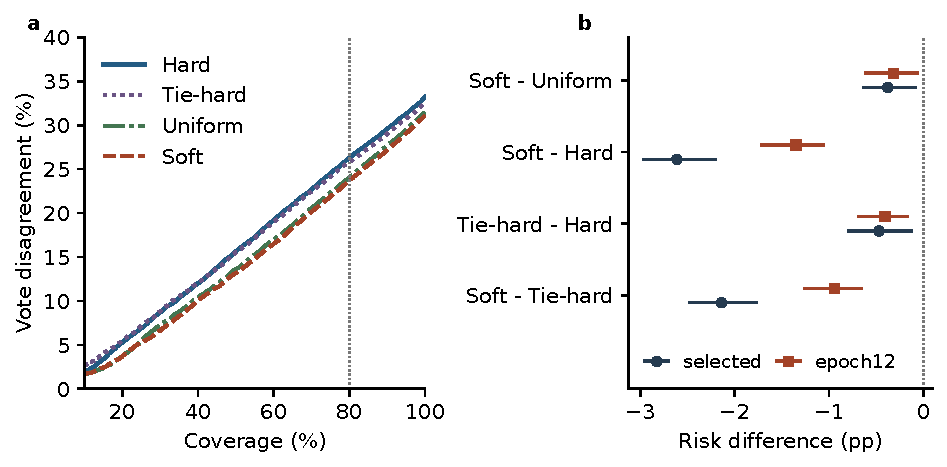
\includegraphics[width=\linewidth]{reviewer_followup/figures/Fig2.pdf}
\caption{(a) Mean selected-checkpoint risk--coverage curves across three seeds; the displayed range begins at 10\%, and every prefix is released. (b) Mean paired contrasts and conditional 95\% pixel-cluster intervals, for selected and epoch-12 weights. Negative differences favor the first-named target. Intervals do not measure seed-population or external-domain uncertainty}\label{fig:contrasts}
\end{figure}
\subsection{Selection sensitivity and label references}
\begin{table}[t]
\caption{Fixed-budget sensitivity and reference-specific metrics. Risk is at 80\% coverage; F1 is at full primary coverage using selected checkpoints. Values are means across three seeds}\label{tab:sensitivity}
\centering\begin{tabular}{lrrrr}\toprule
Targets & Selected & Epoch 12 & Original F1 & Majority F1\\\midrule
Hard & 26.30 & 24.98 & 0.5658 & 0.8965\\
Tie-hard & 25.82 & 24.58 & 0.5599 & 0.9032\\
Uniform & 24.06 & 23.95 & 0.5683 & 0.9205\\
Soft & 23.68 & 23.63 & 0.5722 & 0.9270\\
\bottomrule\end{tabular}
\smallskip\par\footnotesize Risk is a percentage. Both F1 columns are weighted F1, but original labels cover 3,275 images whereas strict crowd-majority labels cover 2,484. Original and crowd-majority labels disagree on 28.46\% of that subset. These F1 values are not interchangeable FER scores. All per-seed values, macro F1, distances, and selected epochs are released.
\end{table}

At fixed epoch 12, Soft minus Uniform is -0.32 pp (conditional 95\% interval [-0.63, -0.05]), and Soft minus Hard is -1.35 pp (conditional 95\% interval [-1.72, -1.05]). Table~\ref{tab:sensitivity} keeps both evaluation states visible. This test changes the stopping decision, not the budget or training objective. The majority-only F1 column concerns a restricted reference task, not an interchangeable performance improvement over original-label F1.

\subsection{Supported mass and the meaning of confidence}
Figure~\ref{fig:mass} separates unsupported mass from ambiguity and excess on each accepted set. Its second panel changes the selection population explicitly rather than silently dropping unsupported votes.
\begin{figure}[t]
\centering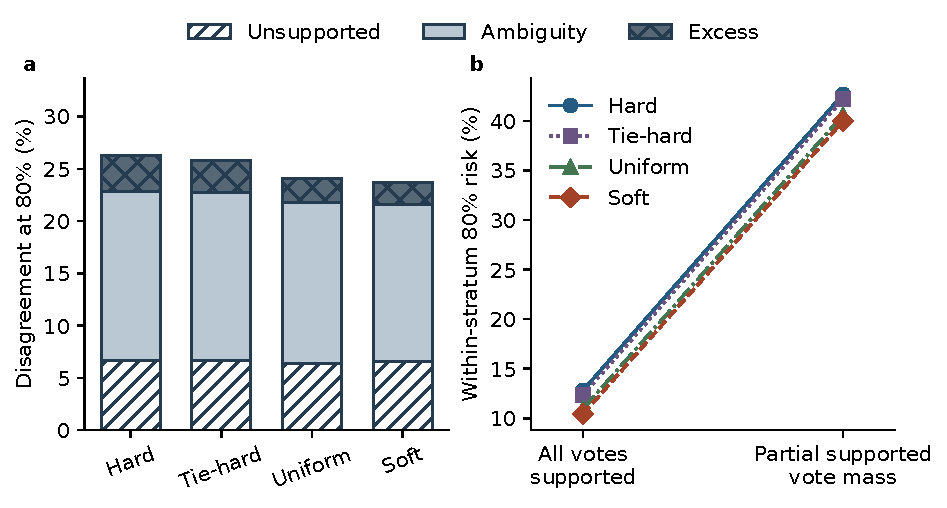
\includegraphics[width=\linewidth]{reviewer_followup/figures/Fig3.pdf}
\caption{(a) Three-way mean risk accounting on global 80\% accepted sets. (b) Independent 80\% selection within full- and partial-supported-mass strata; these populations and vertical scales differ from panel (a). Zero-supported-mass images necessarily have complete-vote risk one and are reported separately in Online Resource 1. Neither panel evaluates an expanded-vocabulary model}\label{fig:mass}
\end{figure}
The primary population contains 1,732 fully supported, 1,527 partially supported, and 16 zero-supported-mass images. Within the fully supported stratum, 80\% risk is 10.42\% for Soft and 10.94\% for Uniform. Within the partially supported stratum, 80\% risk is 40.00\% for Soft and 40.58\% for Uniform. These descriptive comparisons address whether the primary contrast is confined to images with unsupported votes; they do not establish why a model assigned a particular score.

\subsection{Calibration transfer and finite-sample diagnostics}
\begin{table}[t]
\caption{Calibration-fitted policies applied unchanged to primary testing. Entries are mean coverage / risk (\%); coverage includes empty seeds, risk averages nonempty seeds}\label{tab:policies}
\centering\begin{tabular}{llcc}\toprule
Target & Targets & Empirical & Fixed-grid bound\\\midrule
10\% & Hard & 38.35 / 11.45 (3/3) & 0.00 / -- (0/3)\\
10\% & Tie-hard & 39.17 / 11.93 (3/3) & 0.00 / -- (0/3)\\
10\% & Uniform & 45.99 / 12.22 (3/3) & 0.00 / -- (0/3)\\
10\% & Soft & 49.54 / 13.01 (3/3) & 0.00 / -- (0/3)\\
\addlinespace
20\% & Hard & 68.58 / 22.28 (3/3) & 47.03 / 14.55 (3/3)\\
20\% & Tie-hard & 71.04 / 22.80 (3/3) & 48.05 / 14.61 (3/3)\\
20\% & Uniform & 76.20 / 22.80 (3/3) & 57.49 / 16.11 (3/3)\\
20\% & Soft & 76.88 / 22.56 (3/3) & 60.39 / 16.60 (3/3)\\
\addlinespace
30\% & Hard & 98.06 / 32.39 (3/3) & 82.01 / 26.92 (3/3)\\
30\% & Tie-hard & 99.47 / 32.37 (3/3) & 85.41 / 27.54 (3/3)\\
30\% & Uniform & 99.94 / 31.46 (3/3) & 88.41 / 27.11 (3/3)\\
30\% & Soft & 99.91 / 31.07 (3/3) & 89.57 / 27.01 (3/3)\\
\bottomrule\end{tabular}
\smallskip\par\footnotesize Parentheses give nonempty test seeds. An empty policy has undefined risk. Neither a nominal target nor the bound's unverified independence/unchanged-population assumptions establish a deployment guarantee. Different achieved risks are not an equal-risk coverage comparison.
\end{table}

Table~\ref{tab:policies} includes every target and empty-policy outcome. Figure~\ref{fig:transfer} partitions the empirical policy's accepted-population risk change.
\begin{figure}[t]
\centering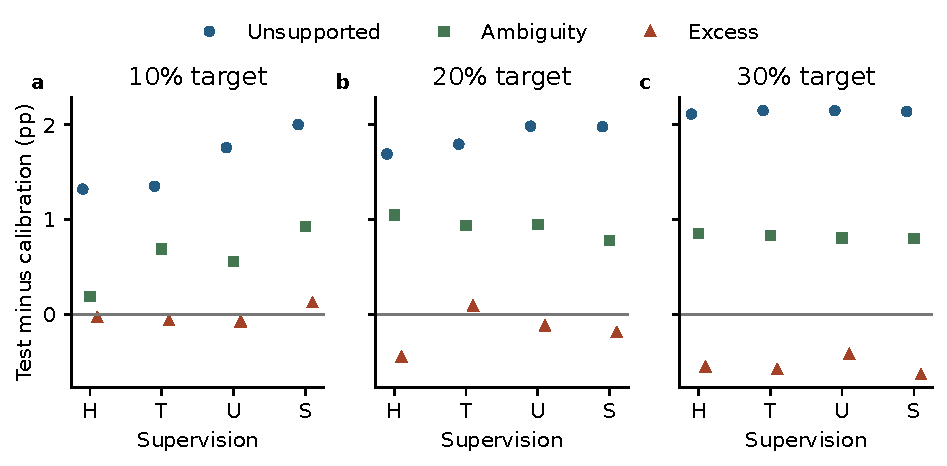
\includegraphics[width=\linewidth]{reviewer_followup/figures/Fig4.pdf}
\caption{Mean test-minus-calibration differences in unsupported mass, supported ambiguity, and excess error for empirical thresholds. Their sum is the risk gap, not a causal attribution. H: Hard; T: Tie-hard; U: Uniform; S: Soft. The three target panels share a vertical scale. Means use paired nonempty calibration/test selections}\label{fig:transfer}
\end{figure}
Across four conditions, 36 of 36 nonempty empirical test operating points exceed their nominal targets. These overlapping outcomes are not independent Bernoulli trials. At the 10\% target, Hard has 38.35\% mean coverage and 11.45\% mean achieved risk. At the 10\% target, Soft has 49.54\% mean coverage and 13.01\% mean achieved risk. Different achieved risks prevent interpreting this as greater coverage at equal risk.

Before confidence selection, the annotation floor is 23.70\% in calibration and 26.67\% in testing: a +2.97 pp difference. Unsupported mass changes from 5.72\% to 7.88\%; the remaining floor difference is supported-category ambiguity. Thus, these populations differ in annotation composition even before a model supplies a ranking.

For Soft at the nominal 20\% target, the accepted test-minus-calibration risk gap is +2.57 pp, comprising +1.98 pp unsupported mass, +0.78 pp supported ambiguity, and -0.19 pp excess. The figure and ledger supply the analogous accounting for every condition and target; this arithmetic does not identify independent causal contributions.

For Hard, the 20\% calibration-half-split holdout-minus-fit risk gap averages +0.05 pp over 300 nonempty seed--split outcomes (descriptive 5th--95th percentiles -2.33 to +2.59 pp). For Tie-hard, the 20\% calibration-half-split holdout-minus-fit risk gap averages +0.18 pp over 300 nonempty seed--split outcomes (descriptive 5th--95th percentiles -2.34 to +2.77 pp). For Uniform, the 20\% calibration-half-split holdout-minus-fit risk gap averages +0.19 pp over 300 nonempty seed--split outcomes (descriptive 5th--95th percentiles -2.02 to +2.62 pp). For Soft, the 20\% calibration-half-split holdout-minus-fit risk gap averages +0.17 pp over 300 nonempty seed--split outcomes (descriptive 5th--95th percentiles -2.00 to +2.43 pp). The complete target-specific resamples are released. These diagnostics reveal within-calibration variability and accepted-population differences, but cannot uniquely separate distribution shift, finite-sample fluctuation, and threshold-search effects.
The fixed-grid comparator yields 24 nonempty test operating points, of which 0 exceed their nominal targets. It abstains completely at the 10\% target for every condition and seed. Its observed conservatism therefore has a concrete coverage cost; these outcomes do not verify its population assumptions.


\section{Discussion}
Full soft targets yielded lower selective disagreement than the ambiguity-preserving uniform-minority control under this matched protocol. This is a test of whether minority allocation supplies added selective value beyond dominant-confidence-preserving softening, not a claim that soft-label learning itself is new. The tie-aware condition directly probes a second alternative explanation rather than adding model capacity. The selected and final-epoch results delimit the dependence on the stopping rule; neither warrants universal superiority.

The size of the control contrast matters: Uniform lowers selected-checkpoint disagreement relative to Hard by 2.23 pp, compared with 2.61 pp for Soft. Thus, the simpler target reproduces much of the observed hard-to-soft difference; detailed minority allocation adds a modest residual advantage under this protocol. This is an endpoint comparison, not a percentage of improvement causally explained by softening.

The vocabulary diagnostics explain why a high supported-class confidence cannot by definition encode all complete-vote risk. Unsupported mass and supported ambiguity are separately observable in the held-out annotations, while MSP omits the former even at the ideal supported-distribution optimum. Nevertheless, observed risk gaps also contain excess category-choice error. The decomposition is useful precisely because it prevents attributing a total change to a single mechanism without evidence.

The conservative grid comparator adds a specified finite-sample margin, at a potential coverage cost. Its assumptions have not been established for deployment or person-level independence in this benchmark, so empirical compliance is not proof of a general guarantee. Calibration half-splits are similarly diagnostic rather than a new validation cohort. The practical recommendation is to report achieved risk, coverage, annotation vocabulary, and accepted-set composition together, instead of treating a nominal confidence policy or majority-only F1 as sufficient reliability evidence.



The distinction in Eq.~\ref{eq:decomposition} is important for interpretation. A lower selected vote-disagreement rate can reflect a lower annotation floor, a lower excess above that floor, or both. Reporting only total risk would conceal these different components. Conversely, the floor is not an immutable property of the person or even the image: it depends on this annotation panel, category vocabulary, and missing conversational context. Extending the vocabulary could change the available-category floor, but that is not what the seven-output experiment tests.

The study addresses a narrower question than whether expression cues improve communication. A model may agree with annotators and still attach a category irrelevant to the sender's intended meaning. Rejecting ambiguous examples may remove precisely the nuance the application aims to retain. Sender control gives an opportunity to suppress a cue, but its benefit and comprehensibility were not evaluated. The prototype is therefore an implementation artifact motivated by the measurement problem, not a validated intervention.

\subsection{Limitations and scope of inference}
The principal limitation is one reused image source. FER+ reannotates FER2013; it is not an independent image dataset. Earlier PrivateTest outcomes informed both experimental phases. The six-control protocol was fixed before its execution but after the hard/soft results and reviewer suggestions were known. Pixel isolation removes a specific overlap route, not identity leakage, near duplicates, dataset-selection bias, or independent-domain uncertainty. The findings are conditional within-dataset evidence rather than external confirmation.

Three paired seeds and a fixed 12-epoch budget constrain optimization claims. Fixed-epoch sensitivity does not establish convergence or insensitivity to all selection criteria. Grayscale preprocessing, small images, architecture, and supported-vote weighting can affect the contrasts. We do not compare a learned selector, another backbone, a second independently acquired vote-annotated image source, or an expanded-vocabulary model. Supported-mass stratification diagnoses the present vocabulary but does not replace such a model experiment. The controls test specific alternative explanations, not all mechanisms behind the observed differences. Favorable results would not establish algorithmic novelty; unfavorable results would not refute distribution learning generally.

Uniform preserves dominant confidence, not target entropy or all class marginals: distributing residual mass uniformly generally changes both. Its contrast with Soft tests these two specified target representations, not a unique causal effect of alternative-category identities or a proof that full distributions are necessary. Tie-hard addresses canonical ties only, not every alternative hard-label construction. The follow-up does not eliminate these remaining design dependencies.

FER images differ from detected faces during message composition. Lighting, pose, occlusion, accessories, camera quality, and detector failures may alter both predictions and rejection behavior. Demographic and cultural variation were not evaluated. The benchmark does not establish mobile efficiency, runtime error bounds, or communication benefit. No participant findings, survey ratings, or interpersonal conclusions are included.

The historical preprint described manual relabeling and reported scores whose curation records and checkpoints were not retained. Those scores are excluded from the new findings; their provenance is documented separately. The current experiment uses traceable public annotations, not an assertion that the historical manual process has been reproduced. Independent-image evaluation and an appropriately reviewed communication study remain distinct future work, rather than evidence supplied by this revision.

\section{Conclusion}
Full soft targets yielded lower selective disagreement than the ambiguity-preserving uniform-minority control under this matched protocol. The primary Soft-minus-Uniform contrast at 80\% coverage was -0.38 pp; its fixed-epoch counterpart was -0.32 pp. The four-condition controls, three-part disagreement accounting, and calibration diagnostics make the limited empirical result interpretable without claiming a new architecture or an operational risk guarantee.


The implemented system preserves sender choice and suppresses invalid or stale observations, while stopping at a local conversation preview. Its scientific relevance is the concrete setting in which annotation-sensitive reliability matters. The present evidence does not establish what a sender feels or whether attaching a cue improves a conversation.

\backmatter
\section*{Statements and Declarations}
\noindent\textbf{Funding.} No funds, grants, or other support were received for preparation of this manuscript.

\noindent\textbf{Competing interests.} The authors declare no competing interests.

\noindent\textbf{Author contributions.} Gunjan Kumar Mishra conceived the prototype and led manuscript preparation. Bijaya Ghimire contributed to implementation, experimental design, and manuscript revision. Badri Raj Lamichhane supervised the work, contributed to methodology review, interpretation, and manuscript revision, and serves as corresponding author. Alan Shah contributed to literature review and code testing. All four authors approved the authorship arrangement and declarations.

\noindent\textbf{Ethics approval.} This work reanalyzes existing benchmark images and annotations and performs software tests. No institutional ethics approval or exemption determination was obtained. The authors do not treat public availability as proof of institutional exemption.

\noindent\textbf{Consent to participate.} No participants were recruited and no new participant data were collected for this revision. Consent documentation for every photograph in the existing benchmark was not independently verified; public availability is not presented as proof of such consent.

\noindent\textbf{Consent for publication.} No identifiable facial photograph is reproduced. Interface illustrations contain synthetic text and no participant images.

\noindent\textbf{Data availability.} Acquisition records for FER2013 \cite{goodfellow2013fer} and official FER+ annotations \cite{barsoum2016ferplus}, immutable hashes, role assignments, and sample-level model probabilities are supplied in Online Resource 1. Images are not redistributed. The full ten-category annotations are retained for auditing the reported metrics.

\noindent\textbf{Code availability.} Online Resource 1 supplies experimental, analysis, and application code, tests, environment records, predictions, and package hashes. Online Resources 2--5 supply selected and epoch-12 inference checkpoints for Hard, Soft, Uniform, and Tie-hard, respectively. The earlier project repository is \url{https://github.com/bijay-gh/face_emotion_embedding}; packaged manifests identify this revision rather than assuming that the public repository contains it. Automated artifact regeneration is an internal verification, not an external replication.

\noindent\textbf{Preprint statement.} An earlier version appeared on TechRxiv as ``Typing with Emotions: Facial Expression Recognition and Embedding in Text Messages,'' version 1, \url{https://doi.org/10.36227/techrxiv.175416003.30236370/v1}. This revision excludes participant evidence and unverifiable historical performance claims, corrects implementation descriptions, and supplies newly documented experiments. It does not claim to reproduce the historical curation procedure.

\noindent\textbf{Supplementary information.} Online Resource 1: code, both protocols, acquisition and split manifests, per-seed predictions and results, supplementary diagnostics, and historical provenance. Online Resources 2--5: all 24 selected and fixed-epoch inference checkpoints, grouped by supervision condition, with checksum manifests.

\bibliography{reviewer_followup/references}
\end{document}
